En esta sección se presenta el artículo de revista publicado en Journal of Information Systems and Applications (JISA) como resultado de la investigación desarrollada en este trabajo.

% Portada del artículo JISA
\begin{figure}[H]
    \centering
    \begin{tcolorbox}[
        colback=white,
        colframe=gray!50,
        boxrule=1pt,
        arc=2pt,
        boxsep=5pt,
        left=3pt,
        right=3pt,
        top=3pt,
        bottom=3pt,
        drop shadow
    ]
        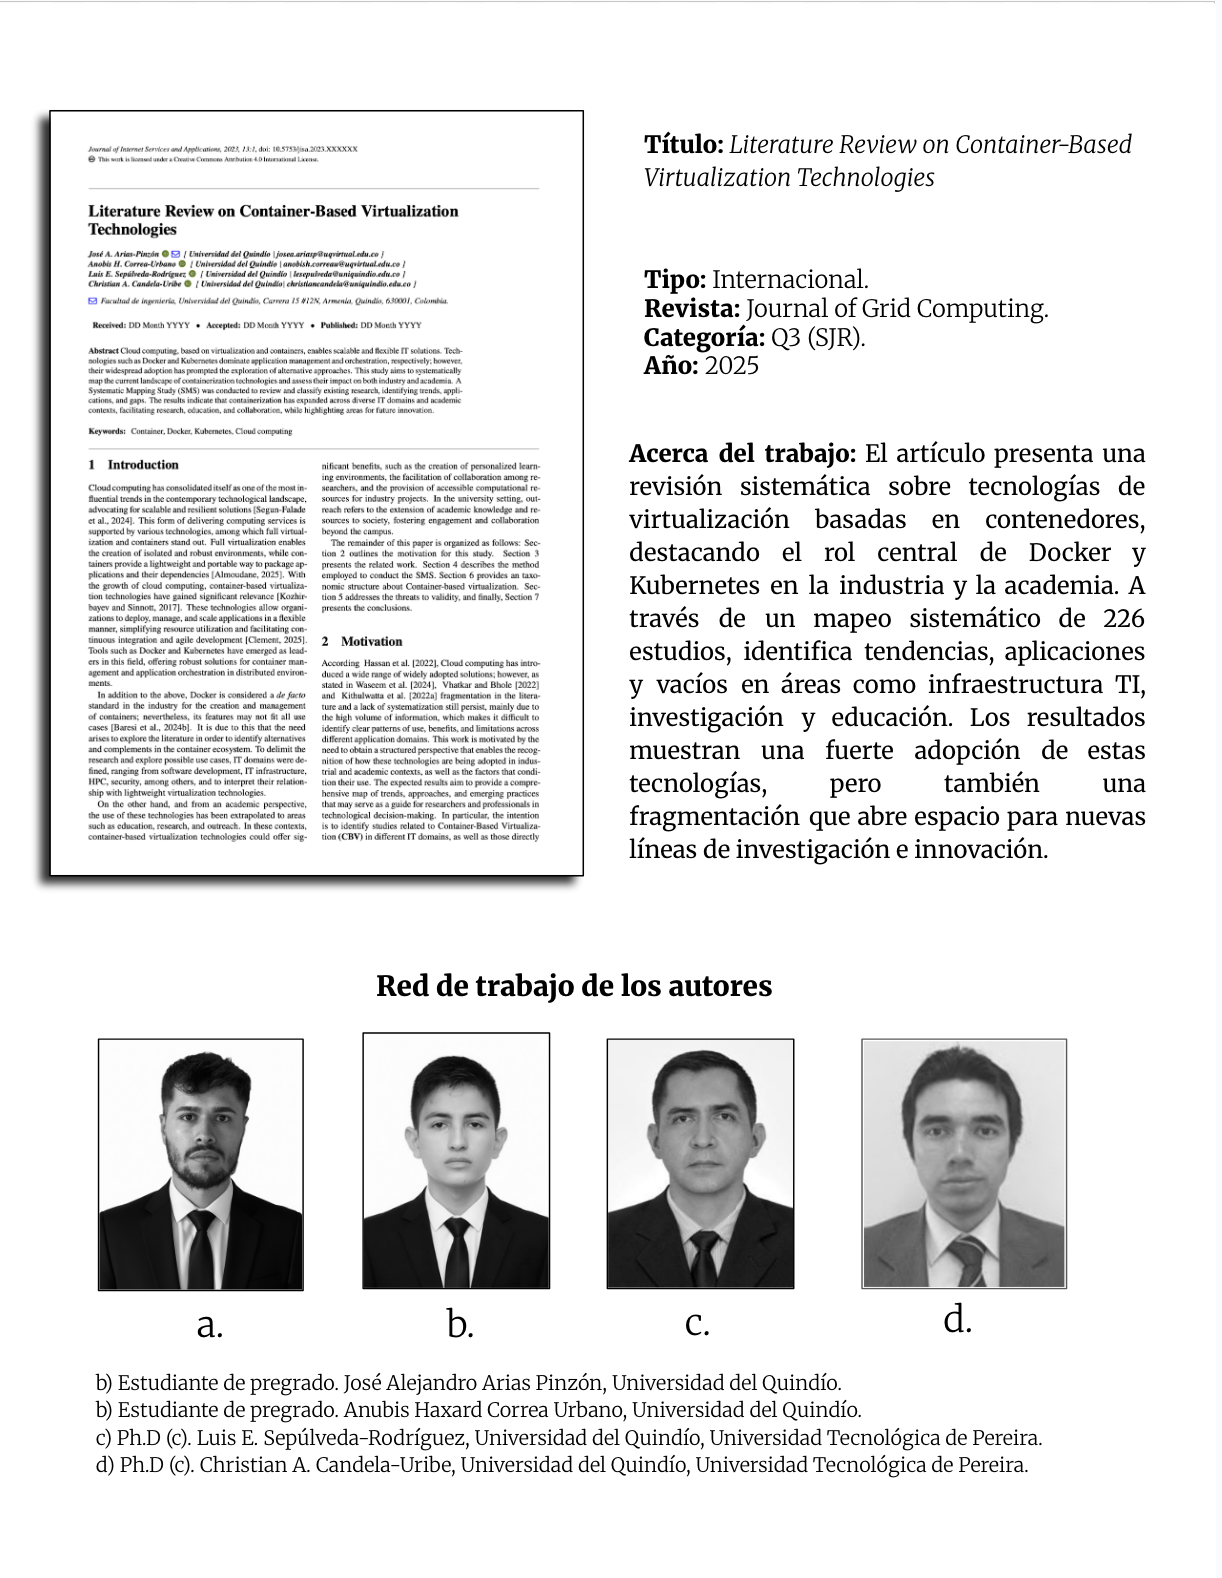
\includegraphics[width=0.95\textwidth,keepaspectratio]{apendices/PORTADA-ART/JISA-PORTADA.png}
    \end{tcolorbox}
    \caption{Portada del artículo JISA}\label{fig:jisa-portada}
\end{figure}
\FloatBarrier

% Página 1
\begin{figure}[H]
    \centering
    \begin{tcolorbox}[
        colback=white,
        colframe=gray!50,
        boxrule=1pt,
        arc=2pt,
        boxsep=5pt,
        left=3pt,
        right=3pt,
        top=3pt,
        bottom=3pt,
        drop shadow
    ]
        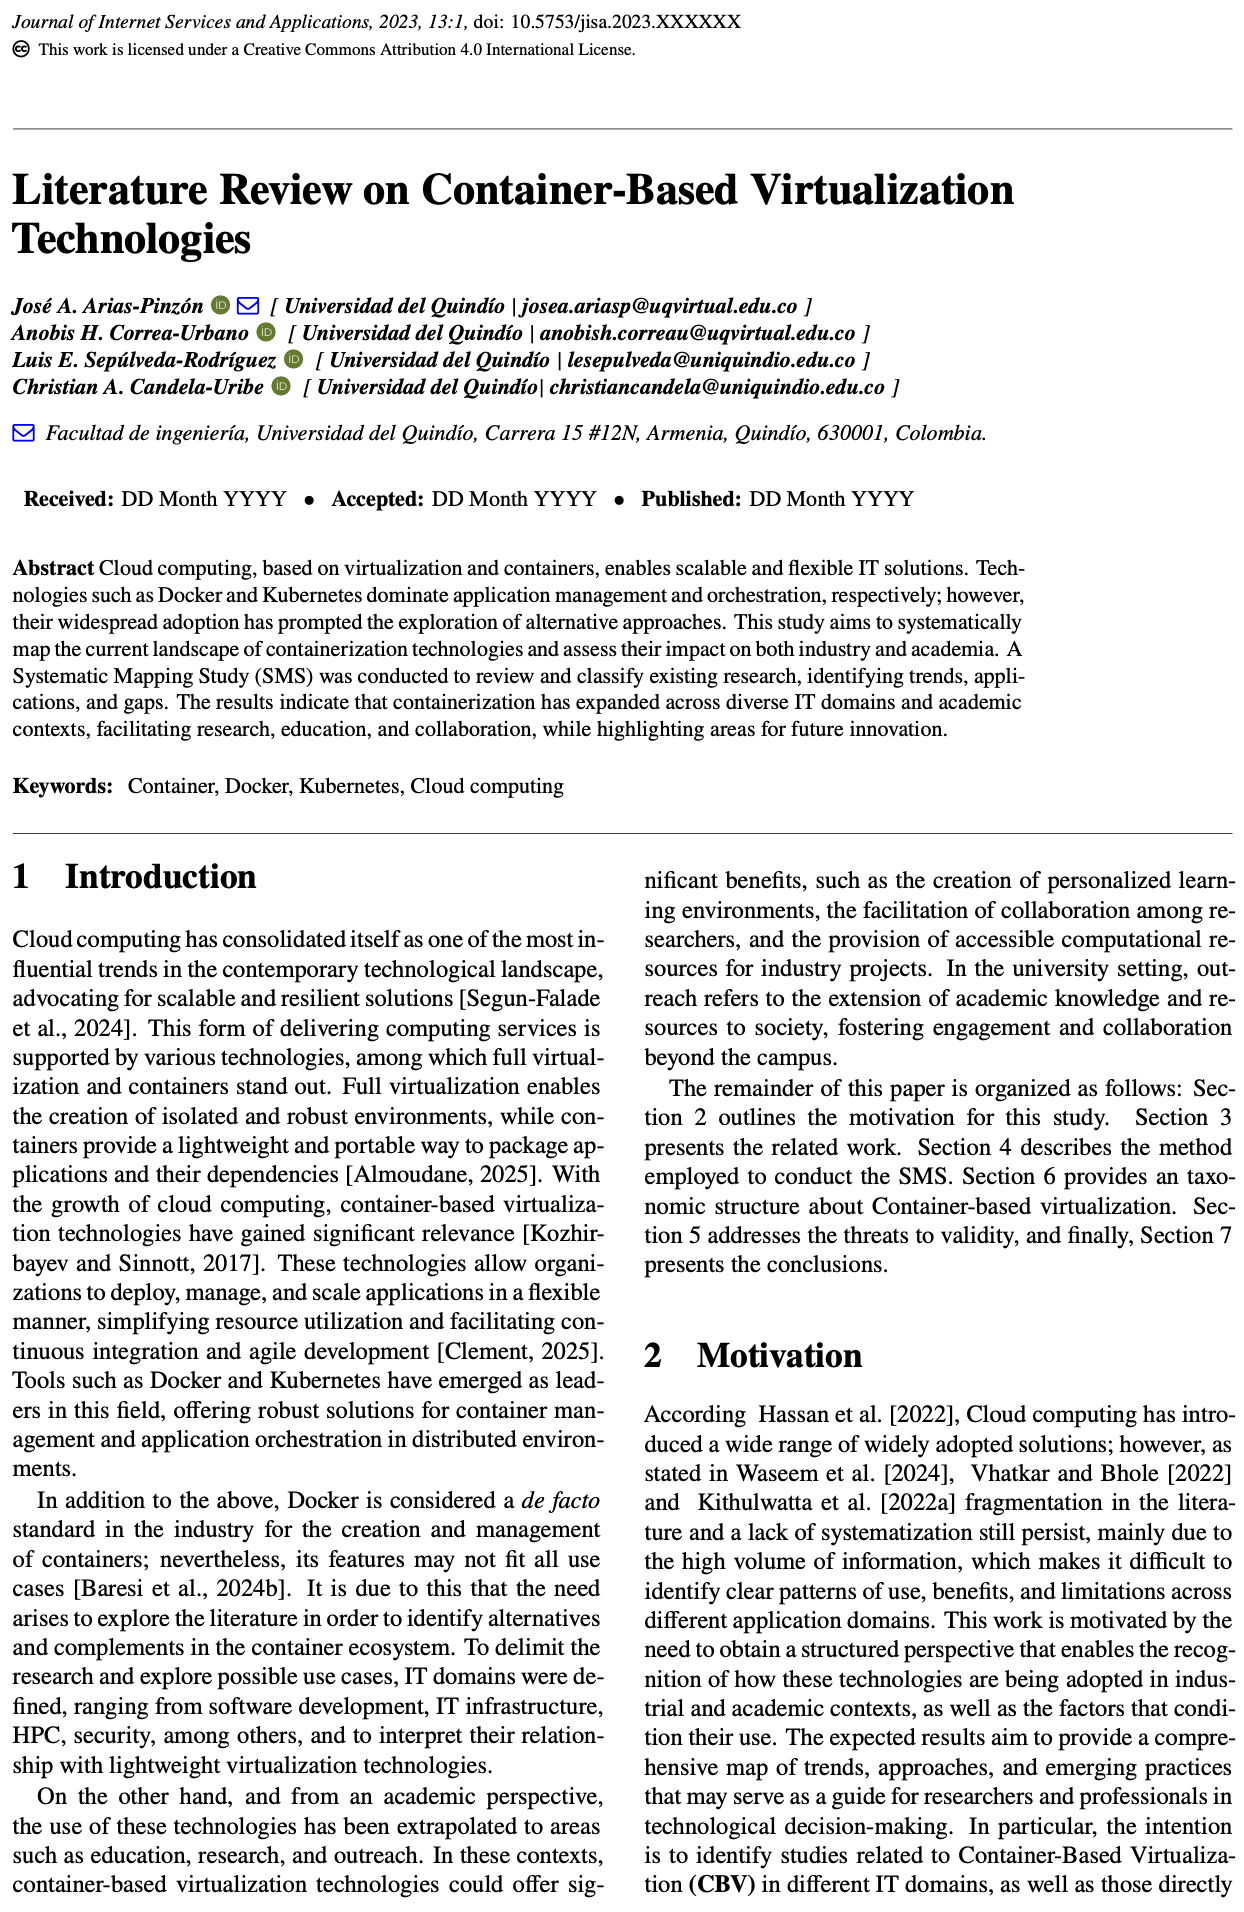
\includegraphics[width=0.95\textwidth,keepaspectratio]{apendices/JISA/pagina_1.png}
    \end{tcolorbox}
    \caption{Artículo JISA --- Página 1}\label{fig:jisa-pagina-1}
\end{figure}
\FloatBarrier% Página 2
\begin{figure}[H]
    \centering
    \begin{tcolorbox}[
        colback=white,
        colframe=gray!50,
        boxrule=1pt,
        arc=2pt,
        boxsep=5pt,
        left=3pt,
        right=3pt,
        top=3pt,
        bottom=3pt,
        drop shadow
    ]
        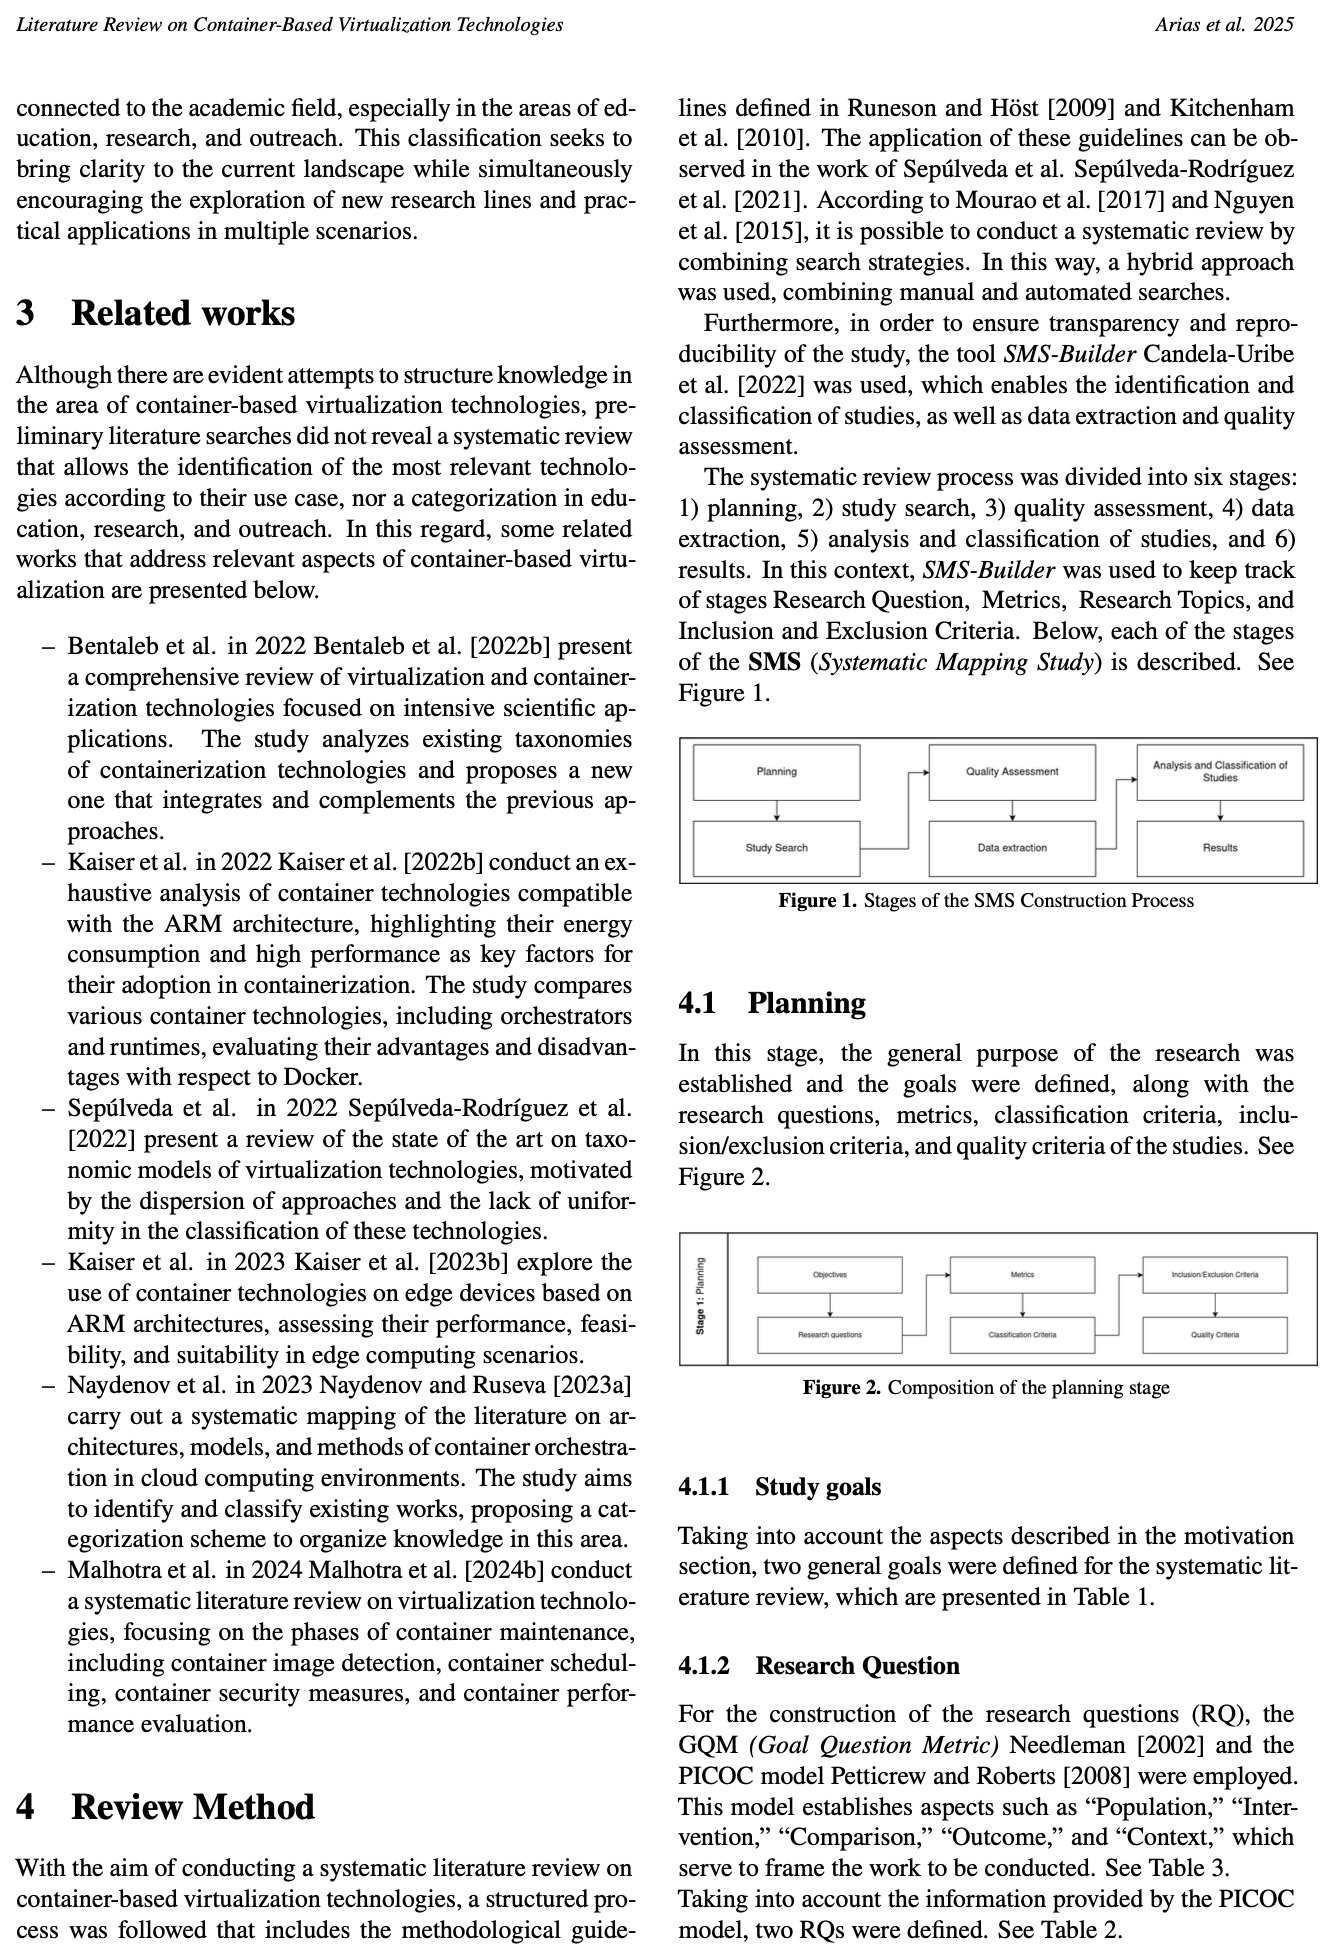
\includegraphics[width=0.95\textwidth,keepaspectratio]{apendices/JISA/pagina_2.png}
    \end{tcolorbox}
    \caption{Artículo JISA --- Página 2}\label{fig:jisa-pagina-2}
\end{figure}
\FloatBarrier% Página 3
\begin{figure}[H]
    \centering
    \begin{tcolorbox}[
        colback=white,
        colframe=gray!50,
        boxrule=1pt,
        arc=2pt,
        boxsep=5pt,
        left=3pt,
        right=3pt,
        top=3pt,
        bottom=3pt,
        drop shadow
    ]
        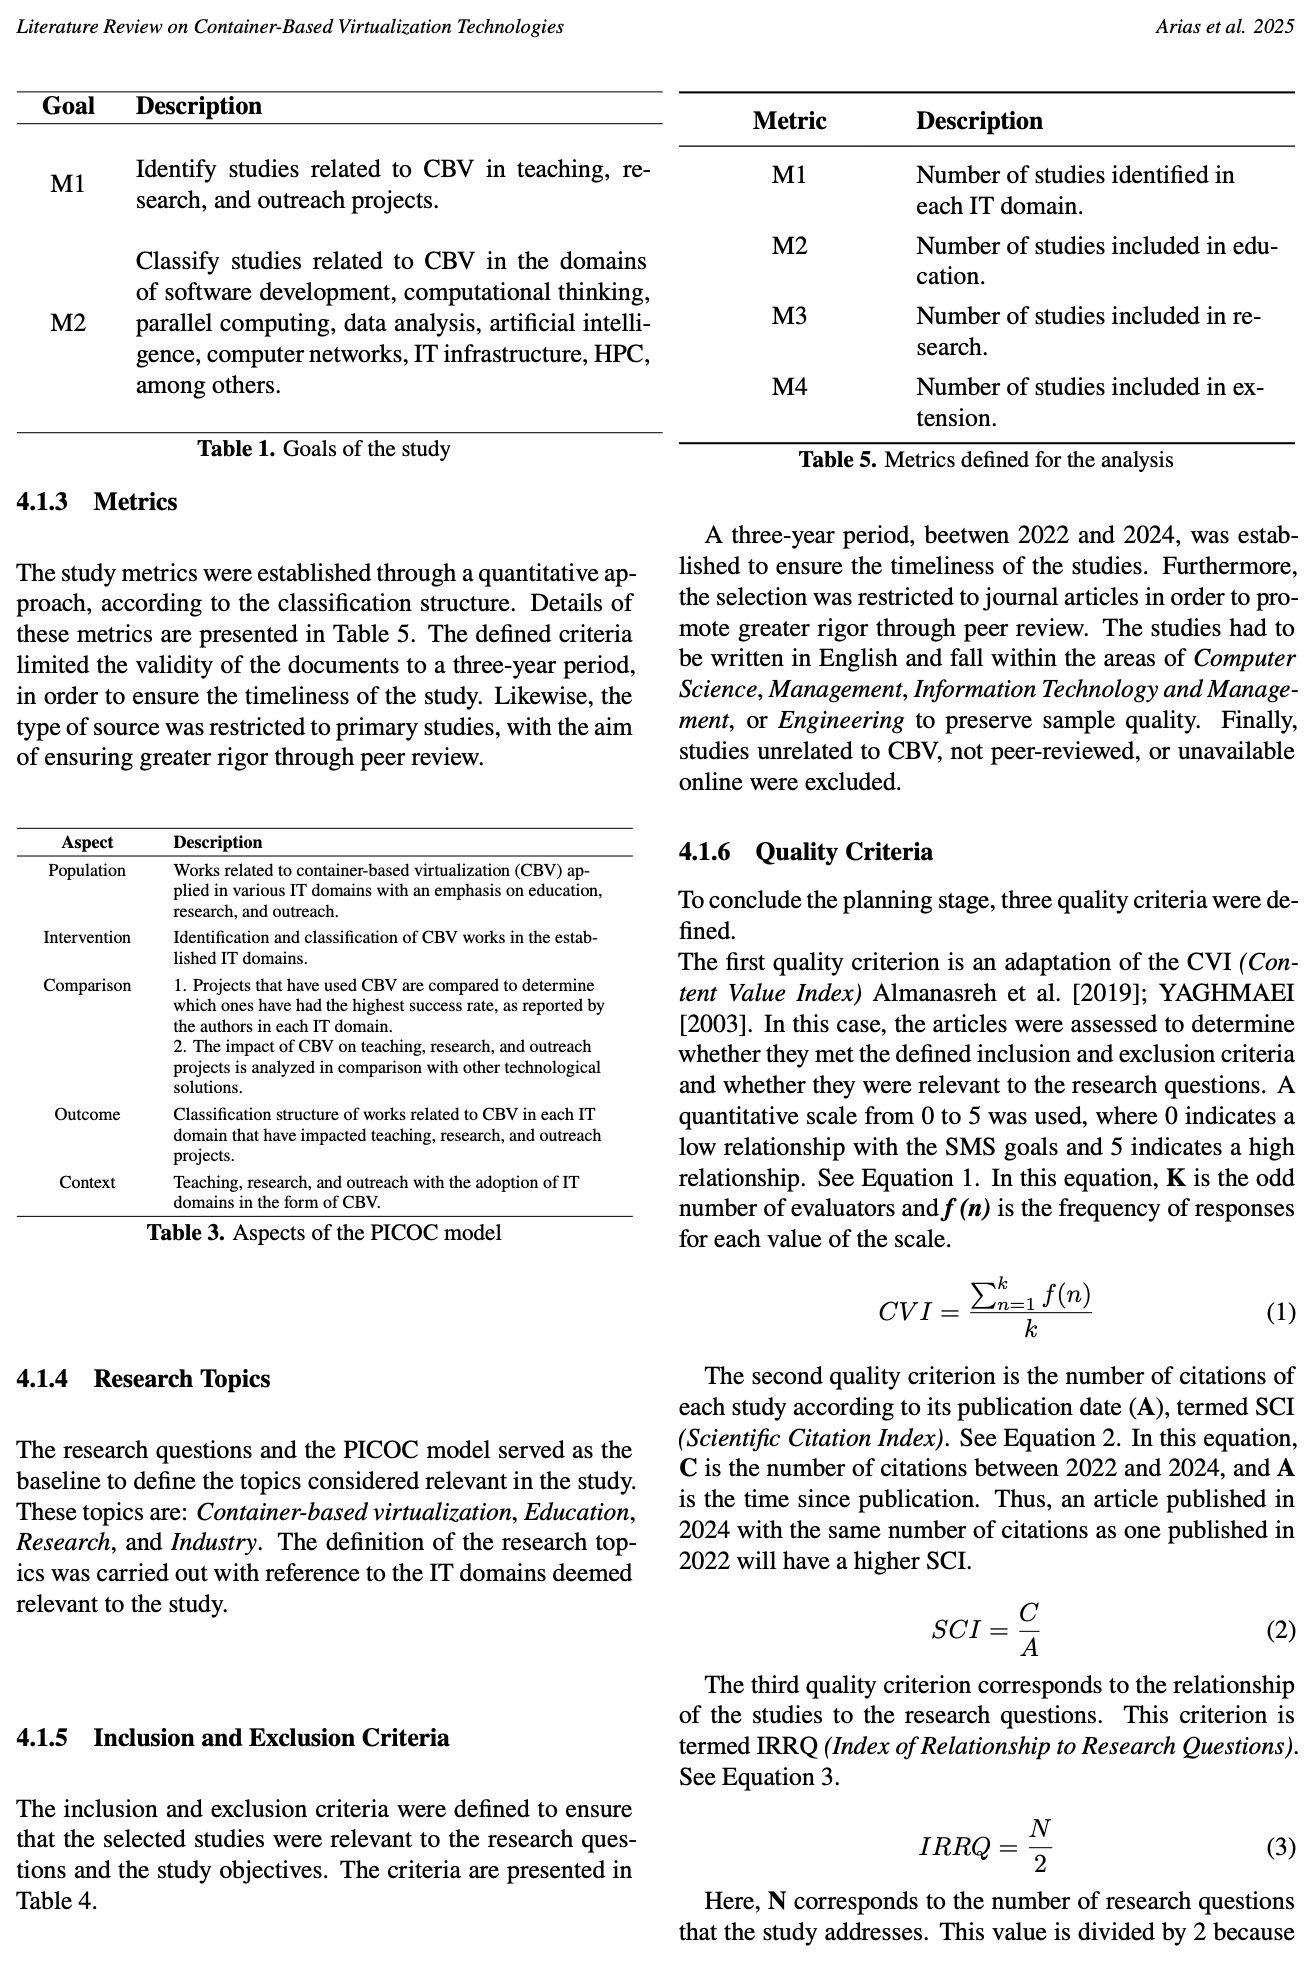
\includegraphics[width=0.95\textwidth,keepaspectratio]{apendices/JISA/pagina_3.png}
    \end{tcolorbox}
    \caption{Artículo JISA --- Página 3}\label{fig:jisa-pagina-3}
\end{figure}
\FloatBarrier% Página 4
\begin{figure}[H]
    \centering
    \begin{tcolorbox}[
        colback=white,
        colframe=gray!50,
        boxrule=1pt,
        arc=2pt,
        boxsep=5pt,
        left=3pt,
        right=3pt,
        top=3pt,
        bottom=3pt,
        drop shadow
    ]
        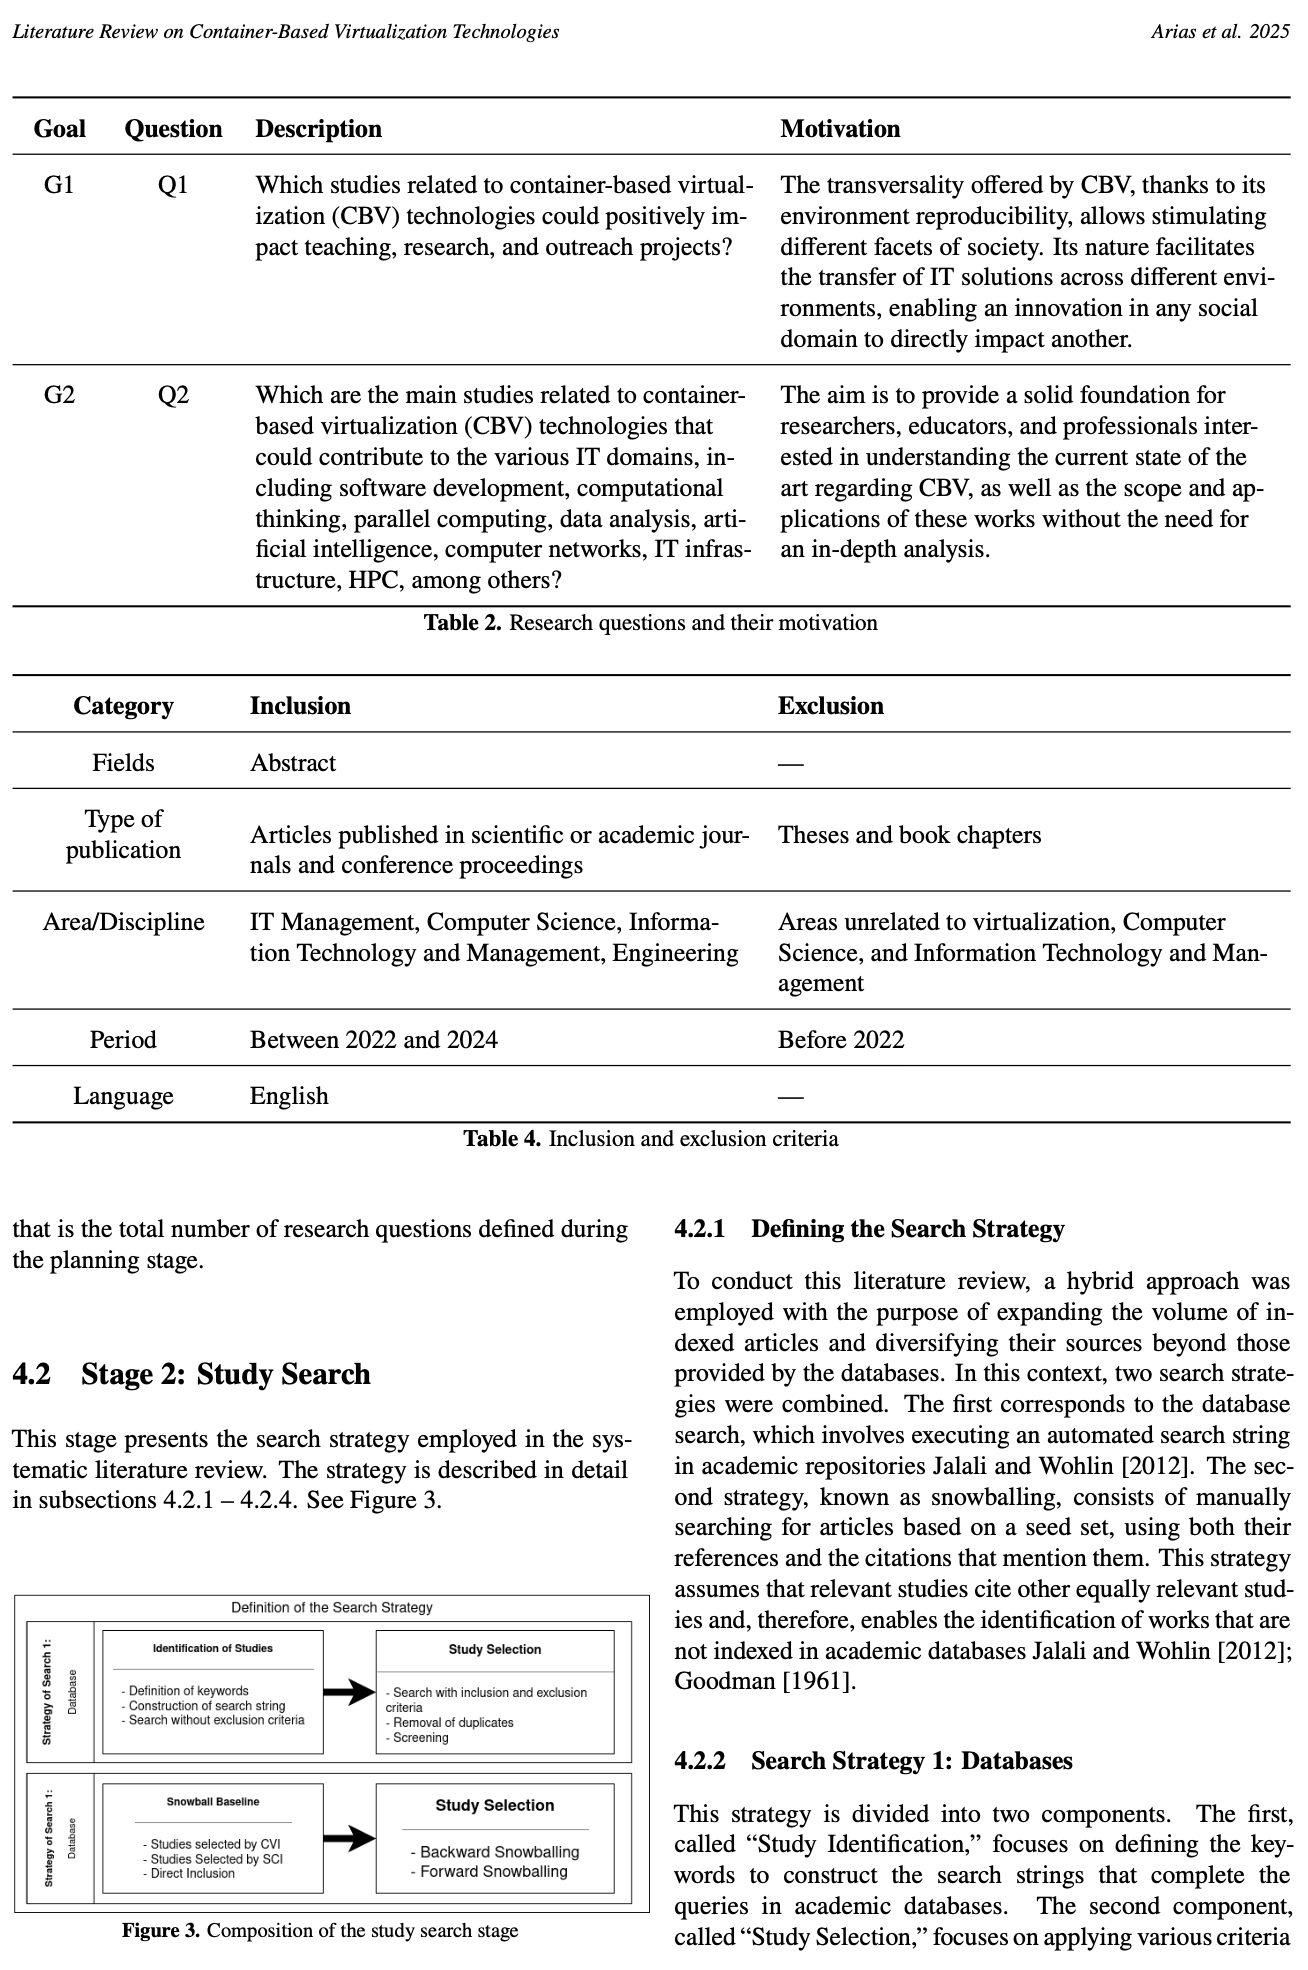
\includegraphics[width=0.95\textwidth,keepaspectratio]{apendices/JISA/pagina_4.png}
    \end{tcolorbox}
    \caption{Artículo JISA --- Página 4}\label{fig:jisa-pagina-4}
\end{figure}
\FloatBarrier% Página 5
\begin{figure}[H]
    \centering
    \begin{tcolorbox}[
        colback=white,
        colframe=gray!50,
        boxrule=1pt,
        arc=2pt,
        boxsep=5pt,
        left=3pt,
        right=3pt,
        top=3pt,
        bottom=3pt,
        drop shadow
    ]
        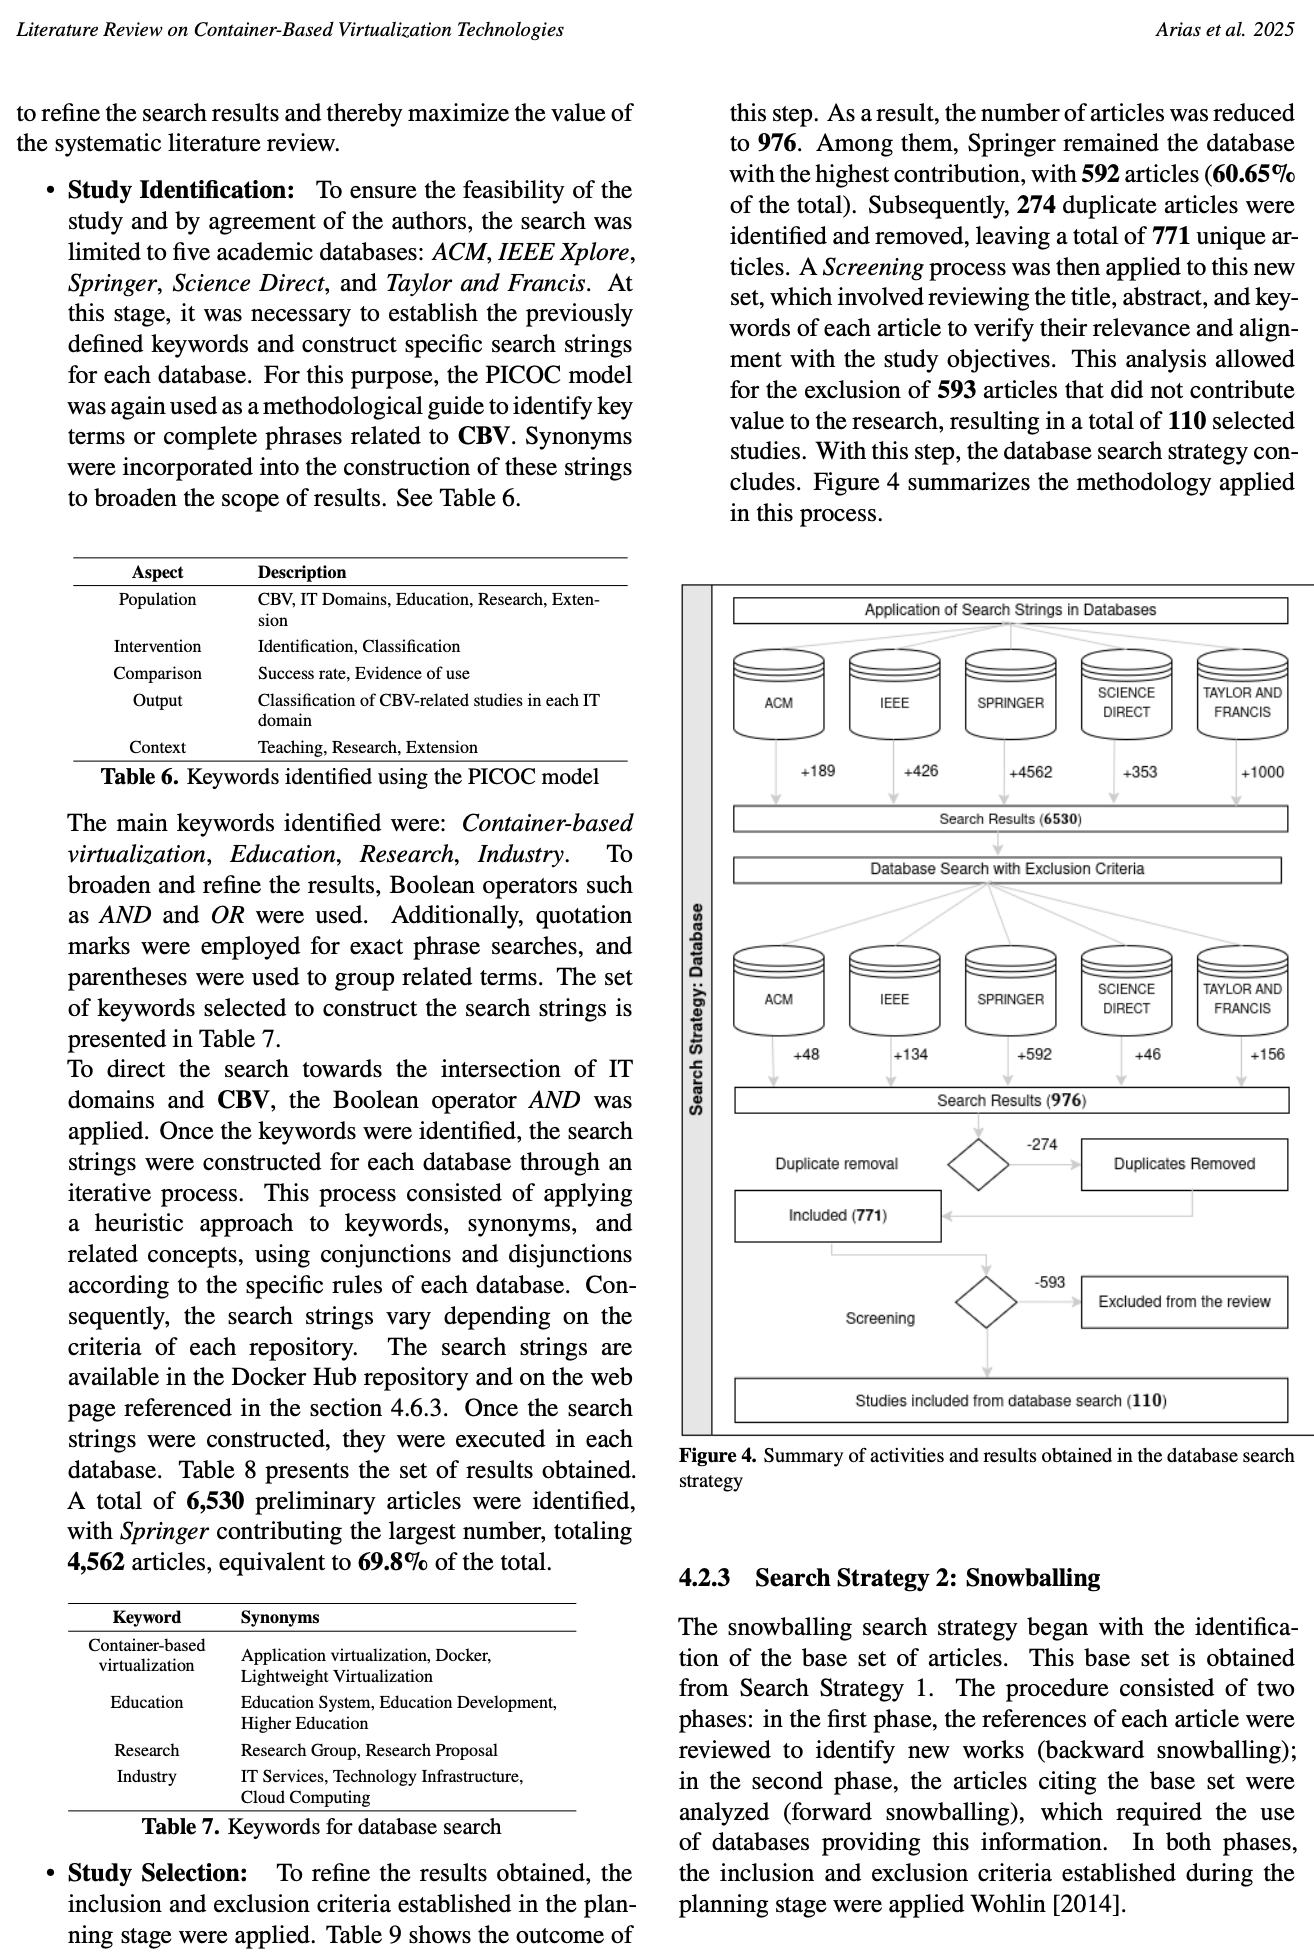
\includegraphics[width=0.95\textwidth,keepaspectratio]{apendices/JISA/pagina_5.png}
    \end{tcolorbox}
    \caption{Artículo JISA --- Página 5}\label{fig:jisa-pagina-5}
\end{figure}
\FloatBarrier% Macro para crear páginas del artículo de forma automática
% Páginas 6-34
\newcounter{jisampage}
\setcounter{jisampage}{6}
\loop%
    \begin{figure}[H]
        \centering
        \begin{tcolorbox}[
            colback=white,
            colframe=gray!50,
            boxrule=1pt,
            arc=2pt,
            boxsep=5pt,
            left=3pt,
            right=3pt,
            top=3pt,
            bottom=3pt,
            drop shadow
        ]
            \includegraphics[width=0.95\textwidth,keepaspectratio]{apendices/JISA/pagina_\thejisampage.png}
        \end{tcolorbox}
        \caption{Artículo JISA --- Página \thejisampage}\label{fig:jisa-pagina-\thejisampage}
    \end{figure}
    \FloatBarrier\stepcounter{jisampage}
    \ifnum\value{jisampage}<35
\repeat%
